\chapter{Basics}
This chapter provides a collection of basic knowledge as a foundation for this work.

\section{Real Time Operating Systems}
\label{sec:rtos}
A \ac{RTOS} is designed with precise timing and high reliability in mind for running applications \textcite{stankovicRealtimeOperatingSystems2004}.
Such systems are used in a wide range of applications, from multimedia systems and smart home systems to automotive and medical sectors, such as pacemakers \cite{hambardeSurveyRealTime2014}.
In all these systems, the correctness and timeliness of the applications are of utmost importance \cite{hambardeSurveyRealTime2014}.
\subsection{Tasks and Jobs}
\label{sec:tasks_and_jobs}
According to the \citetitle{IEEEStandardRealTime}, a task is defined as the "basic logical unit of concurrent program execution" that contains code. The standard also states that while the code within a task is executed sequentially, the tasks themselves may run in parallel with other tasks.

Tasks can have deadlines based on their importance and the nature of their work. If a task misses its deadline due to insufficient computational time, the system and results may be affected differently. It is common to categorize task deadlines into three types \cite{dengSchedulingRealtimeApplications1997,abeniIntegratingMultimediaApplications1998,shindeComparisonRealTime2017}:
\begin{enumerate}
	\item \textbf{Hard Deadline:}
	      Missing a hard deadline is considered a system failure. The task must complete by its deadline; otherwise, the system may enter an unsafe state.
	\item \textbf{Firm Deadline:}
	      Missing a firm deadline does not cause a system failure, but the task's result is no longer useful and is discarded. The system continues to operate, but the quality of service may degrade.
	\item \textbf{Soft Deadline:}
	      Missing a soft deadline reduces the task's utility, but the result can still be used. The system can tolerate some deadline misses without significant impact on overall performance.
\end{enumerate}

\subsection{Real-time Scheduling}
\label{sec:scheduling}
Creating the schedule of given tasks to be executed some aspects

Generating a task set with known \ac{WCET} and \ac{WCRT} requires knowledge about the schedule.
Implementing a scheduler gives the benefit of taking direct insights in the compilation of the generated results. 
To determine the order of operation when being confronted with two or more tasks, the tasks need to get a priority assigned.

There are some scheduling techniques to determine the priority of tasks to be scheduled.
\begin{itemize}
	\item \textbf{Clock based Scheduling:}
	      With clock based scheduling every task gets a share of execution time in which the work of the task may be done.
	      It is a way to schedule tasks without priorities whilst making sure every task gets time on the computational unit.
	      While being a simple algorithm it does create a lot of overhead, since the timeslots do not necessarily encompass the whole time needed by the task.
	\item \textbf{(Weighted) Round Robin:}
	      In basic Round Robin scheduling, each task is assigned a fixed time slice or quantum in a cyclic order, ensuring all tasks get an equal share of CPU time. Weighted Round Robin extends this by assigning different weights to tasks, allowing tasks with higher weights to receive more CPU time compared to tasks with lower weights. This provides a more flexible and efficient scheduling mechanism, especially for systems with tasks of varying importance or computational needs. \cite{helmyOptimizingRoundRobinScheduling2024}
	\item \textbf{Rate Monotonic Scheduling:} Rate monotonic scheduling is a fixed priority algorithm where tasks with shorter periods are assigned higher priorities. It is optimal for fixed priority scheduling under certain conditions. \cite{lehoczkyRateMonotonicScheduling1989}
	\item \textbf{Earliest Deadline First:} With the earliest deadline first scheduling algorithm, the priority of the tasks is not fixed, but dynamic. As the name implies, the tasks get a priority assigned in a way to ensure the tasks with the nearest upcoming deadline get to run first. \cite{lehoczkyPerformanceRealtimeBus1986}
\end{itemize}

\section{Timing Analysis}
\label{sec:timing_analysis}
For real-time systems it is desired to keep up the reliability and predictability of the given tasks to ensure their timely execution respectively to their deadlines.
To deduce a task's worst execution time without underestimating, \ac{WCET} analysis is employed.
Various approaches are currently used to determine the possible execution times of tasks, including static analysis, measurement-based analysis, and probabilistic analysis, which will be discussed in the upcoming sections \cref{sec:static_analysis,sec:measurement_analysis,sec:probabilistic_analysis}.

\subsection{Static Analysis}
\label{sec:static_analysis}
Static analysis makes use of several techniques to generate a model of the given hardware and software to gain knowledge about the executional behavior of the inspected code.
One key benefit of the static analysis is that the code does not need to be executed.

\textcite{wilhelmWorstcaseExecutiontimeProblem2008} describe the static analysis in multiple phases.
These phases are \textit{control-flow analysis}, \textit{processor behavior analysis} and \textit{path analysis}.

\subsubsection{Control-Flow Analysis}
\label{sec:cfa}

\begin{figure}[h]
	\begin{subfigure}[c]{0.45\textwidth}
		\begin{lstlisting}[language=Java,firstnumber=1]
void collatzConjecture(int n) {
  while (n != 1) {
    if (n % 2 == 0) {
      n = n / 2;
    } else {
      n = 3 * n + 1;
    }
    System.out.println(n);
  }
}
\end{lstlisting}
		\caption{Collatz Conjecture Code}
		\label{fig:collatz_code}
	\end{subfigure}
	\hfill
	\begin{subfigure}[c]{0.45\textwidth}
		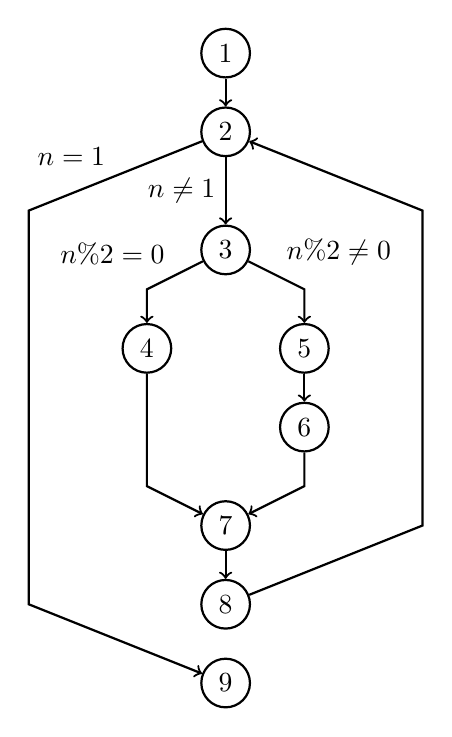
\begin{tikzpicture}
	\node[circle, draw, thick] (n1) at (0, 0) {1};
	\node[circle, draw, thick] (n2) at (0, -1) {2};
	\node[circle, draw, thick] (n3) at (0, -2.5) {3};
	\node[circle, draw, thick] (n4) at (-1, -3.75) {4};
	\node[circle, draw, thick] (n5) at (1, -3.75) {5};
	\node[circle, draw, thick] (n6) at (1, -4.75) {6};
	\node[circle, draw, thick] (n7) at (0, -6) {7};
	\node[circle, draw, thick] (n8) at (0, -7) {8};
	\node[circle, draw, thick] (n9) at (0, -8) {9};

	\draw[->,thick] (n1) -- (n2);
	\draw[->,thick] (n2) -- (n3) node[midway,anchor=east] {$n\ne1$};
	\draw[->,thick] (n2) -- (-2.5,-2) node[midway,anchor=south east,fill=white] {$n=1$} -- (-2.5,-7) -- (n9);
	\draw[->,thick] (n3) -- (-1,-3) node[midway,anchor=south east,fill=white] {$n\%2=0$} -- (n4);
	\draw[->,thick] (n3) -- (1,-3)node[midway,anchor=south west,fill=white] {$n\%2\ne0$} -- (n5);
	\draw[->,thick] (n5) -- (n6);
	\draw[->,thick] (n4) -- (-1,-5.5) -- (n7);
	\draw[->,thick] (n6) -- (1,-5.5) -- (n7);
	\draw[->,thick] (n7) -- (n8);
	\draw[->,thick] (n8) -- (2.5,-6) -- (2.5,-2) -- (n2);
\end{tikzpicture}
		\caption{\ac{CFG} for \cref{fig:collatz_code}}
		\label{fig:cfg}
	\end{subfigure}
	\caption{Example code showing the calculation of the Collatz conjecture and its representation with a \acf{CFG}.}
	\label{fig:collatz_and_cfg}
\end{figure}

When analyzing a given task, a \ac{CFG} is built to represent the execution paths of the task's code, including a task's call graph. The control-flow analysis, previously called \textit{high-level analysis}, attempts to gain as much knowledge about the control flow of a given task by identifying loops and their bounds, flow branches, and function calls. When including information about the data flow of the task, it may be possible to exclude paths from the \ac{CFG} that are infeasible and may not be executed at all, for example, paths with mutually exclusive conditions. 

\Cref{fig:collatz_and_cfg} illustrates an example code snippet for calculating the Collatz conjecture and its corresponding \ac{CFG}. The code snippet, shown in \cref{fig:collatz_code}, contains loops and branches that determine the sequence of operations based on the value of the input number. The \ac{CFG}, depicted in \cref{fig:cfg}, visually represents these control structures, highlighting the possible execution paths, including the loop involving nodes 2, 8, and 9, and a branch divergence between nodes 3 and 7 depending on the current value of $n$.

\todo{flow facts Chen 04 20/83}

\subsection{Data Flow Analysis}
\label{sec:dfa}
\ac{DFA} is 

\todo{timing accidents - Chen 04 10/53}
Key techniques used in static analysis include:
\begin{itemize}
	\item \textbf{Control Flow Analysis:} This technique involves constructing a control flow graph (CFG) of the program, which represents all possible paths that the program execution can take. Nodes in the CFG represent basic blocks of code, and edges represent the flow of control between them.
	\item \textbf{Data Flow Analysis:} This technique analyzes the flow of data within the program to determine how values are propagated and transformed. It helps in identifying dependencies and potential bottlenecks in the code.
	\item \textbf{Abstract Interpretation:} This technique involves creating an abstract model of the program that simplifies its behavior while preserving essential properties. The abstract model can use various representations, including control flow graphs, to analyze and derive bounds on execution times and other properties.
	\item \textbf{Path Analysis:} This technique involves identifying and evaluating all possible execution paths in the program. It helps in determining the longest path, which corresponds to the WCET
	.
\end{itemize}

Static analysis is advantageous because it does not require actual execution of the code, making it suitable for early stages of development. However, it can be overly conservative, leading to pessimistic WCET estimates due to the need to account for all possible execution paths and hardware behaviors.

\subsection{Measurement-based Analysis}
\label{sec:measurement_analysis}

\subsection{Probabilistic Analysis}
\label{sec:probabilistic_analysis}

Early flowcharts and \ac{AI}s describes by \textcite{cousotAbstractInterpretationUnified1977}

\todo{cache misses}
\todo{overestimation \& pessimism}

\begin{figure}[htbp]
	\centering
	\resizebox{\textwidth}{!}{
		\begin{tikzpicture}
	% Axes
	\draw[->,thick] (0,0) -- (20,0) node[below,anchor=north east]{time};
	\draw[->,thick] (0,0) -- (0,5.5) node[left,rotate=90,anchor=south east]{distribution of times};

	% Execution time distribution (just shape some)
	\draw[thick, fill=black!60, pattern=dots] plot[smooth] coordinates {
	(1,0)
	(2,1)
	(3,1.4)
	(4,3.75)
	(5,3.2)
	(6,1.1)
	(7,2.2)
	(8,0.3)
	(9,0.25)
	(10,0.8)
	(11,0.12)
	(12,0.25)
	(13,0)
	} -- (13,0) -- cycle;
	\draw[thick, fill=black!60, pattern=dots] plot[smooth] coordinates {
	(15,0)
	(16,0.3)
	(16.7,0.3)
	(17,0)
	} -- (17,0) -- cycle;
		% measured times
	\draw[thick, fill=black!30, pattern=crosshatch] plot[smooth] coordinates {
	(3,0)
	(4,2.5)
	(5,1.4)
	(6,0.6)
	(7,1.3)
	(8,0.1)
	(9,0.08)
	(10,0.6)
	(11,0.03)
	} -- (11,0) -- cycle;

	% Vertical markers for BCET, min/max observed times, WCET
	\draw[] (0.5,-1.75) -- (0.5,5.5);
	\node[above,fill=white,align=center,rotate=90,anchor=center] at (0.5,2) {Lower bound};
	\draw[] (1,-1.25) -- (1,5.5);
	\node[above,fill=white,align=center,rotate=90,anchor=center] at (1,2) {BCET};
	\draw[] (3,-0.75) -- (3,5.5);
	\node[above,fill=white,align=center] at (3,5) {Minimal\\observed\\execution\\time};
	\draw[] (11,-0.75) -- (11,5.5);
	\node[above,fill=white,align=center] at (11,5) {Maximal\\observed\\execution\\time};
	\draw[] (17,-1.25) -- (17,5.5);
	\node[above,fill=white,align=center,rotate=90,anchor=center] at (17,2) {WCET};
	\draw[] (19,-1.75) -- (19,5.5);
	\node[above,fill=white,align=center,rotate=90,anchor=center] at (19,2) {Upper bound};

	% Horizontal worst-case performance and guarantee
	\draw[line width=0.7mm,->] (0,4.85) -- (14,4.85) node[midway,above]{worst-case performance} -- (17,4.85);
	\draw[line width=0.7mm,->] (0,4.15) -- (14,4.15) node[midway,above]{worst-case guarantee} -- (19,4.15);

	% Execution time arrows
	\draw[<->] (3,-0.5) -- (11,-0.5) node[midway,fill=white]{measured execution times};
	\draw[<->] (1,-1) -- (3,-1) -- (11,-1) node[midway,fill=white]{possible execution times} -- (17,-1);
	\draw[<->] (0.5,-1.5) -- (3,-1.5) -- (11,-1.5) node[midway,fill=white]{timing predictability} -- (19,-1.5);

	% Annotations
	\draw[->, thick] (13,3) -- (15.9,0.7);  
		\node[draw, fill=white, align=center] at (13,3) {The actual WCET\\ must be found or\\ upper bounded};
	
\end{tikzpicture}
	}
	\caption{
		The graph above illustrates two curves representing the basic concepts of timing analysis.
		The first curve, with the dotted area, shows the range of all possible execution times, with the minimum and maximum values being the \ac{BCET} and \ac{WCET}, respectively.
		The second curve, with the crosshatched area, represents the range of execution times identified through analysis, with the minimum and maximum values being the \textit{minimal observed execution time} and \textit{maximal observed execution time}.
		This graph is adapted from \textcite{wilhelmWorstcaseExecutiontimeProblem2008}.
	}
	\label{fig:overestimation}
\end{figure}

\textcite{kelterWCETAnalysisOptimization} mentions several techniques that can be used for \ac{WCET} analysis, including static analysis, measurement-based analysis, statistical analysis and hybrid approaches.
Static analysis involves analyzing the code without executing it, while measurement-based analysis involves running the code on the target hardware and measuring the execution times.
Hybrid approaches combine both static and measurement-based techniques to provide more accurate \ac{WCET} estimates.

Static analysis is a proper and safe way to get information about the execution times, since it is unhinged from hardware constraints and derived from a meta model created from reviewing the code \cite{kelterWCETAnalysisOptimization}.

To evaluate analysis techniques benchmarks play a significant role.
Providing multiple task sets with known execution scenarios and the tasks behavior the analysis techniques can be tested for its effectiveness. 
Benchmarks commonly used are for example the Mälardalen \ac{WCET} benchmark and the TACLeBench benchmark suite \cite{falkTACLeBenchBenchmarkCollection2016}.

Accurate \ac{WCET} analysis is critical for the design and verification of real-time systems, ensuring that all tasks can be scheduled and executed within their deadlines, thereby maintaining the system's overall reliability and performance \cite{kelterWCETAnalysisOptimization}.
\textcite{kelterWCETAnalysisOptimization} states further that \ac{WCET} analyses are no longer sufficient for newer and complex systems and need to analyze delays and preemptions between tasks as well, resulting in \ac{WCRT}.

\subsection{Critical Instant Theorem}
\label{sec:critial_instant_theorem}
The Critical Instant Theorem, introduced by \textcite{liuSchedulingAlgorithmsMultiprogramming1973}, states that the worst-case response time of a task occurs when it is released simultaneously with all higher-priority tasks.
This theorem is fundamental in fixed-priority scheduling, as it helps in determining the worst-case scenario for task execution.

According to the theorem, to find the worst-case response time of a task, one must consider the scenario where the task is released at the same time as all higher-priority tasks. 
This situation is known as the critical instant. By analyzing the system under this condition, one can ensure that the calculated response times are indeed the worst-case values.

The theorem is particularly useful in the context of \ac{RMS} and other fixed-priority scheduling algorithms, as it provides a systematic way to evaluate the schedulability of tasks. 
If all tasks meet their deadlines under the critical instant scenario, the system is considered schedulable.

\subsection{Related Work}
\label{sec:related_work}
\todo{}
\cite{dar-tzenpengAssignmentSchedulingCommunicating1997} Built taskgraph with harmonic set 